\epigraph{``It is our choices, Harry, that show what we truly are, far more than our abilities."}{Albus Dumbledore}

The previous chapters have discussed the development of an open source implementation to simulating atmospheric dynamics both in the troposphere and the stratosphere on a synoptic scale. Although extremely time consuming, and with a few approximations made along the way, the importance of an open source implementation cannot be understated. It could potentially open up a field to a wider group, and often doesn't receive the media attention it rightfully deserves.

Future applications of this work are extremely wide ranging, from usage in numerical weather prediction schemes that take in observational data collected from satellites, and ground stations in order to provide a picture of future weather events; to forming at starting point in future research of atmospheric phenomena, ideally reducing the overall research time. While, at the moment, it definitely would be inaccurate to say the software is ready for such usage, with future enhancements which I will touch on in a minute, it most certainly will.

\section{Looking Back}
To prove the hypothesis that `it is possible to create open source implementation to simulating atmospheric dynamics both in the troposphere and the stratosphere, that such a software is consistent and reliable, and that the software consists of high quality code', a number of different bechmarking experiments were carried out in the areas of: performance, accuracy, and code quality.

It is clearly possible to create open source software implementation to simulating atmospheric dynamics, as evident by this report. In regards to performance benchmarking, two different benchmarks were carried out. The statistical analysis of the first benchmark indicated that the p-value of the null hypothesis was 0.0009, and hence therefore, we can reject the null hypothesis. This demonstrated that there was a significantly significant increase in execution time between the Python version of the software and the Cython version. The statistical analysis of the second benchmark found that the mean coefficient of variation ($\frac{\sigma}{\bar{x}}$) in regards to execution time was approximately, 0.04. This signified that there was a low variation in execution time, proving that the performance of the software was consistent and reliable. In regards to the accuracy benchmark, a mean absolute percentage error of approximately 1.56 \%, and a median absolute percentage error was approximately 0.81 \% were found. This shows that the forecast produced by the software is accurate, and proves that the software is consistent and reliable. In regards to the code accuracy benchmark, two distinct benchmarks were carried out. The first benchmark indicated that the software consists of high quality source code, as it received a numerical rating of 7.32 from Pylint which corresponds to an interpretation of `Great Code!' in table 6.3. The second benchmark indicated that the software had a code coverage of approximately 98 \%. This signifies that the software has a lower chance of containing undetected bugs, ultimately demonstrating that the quality of the source code is high. Both of these benchmarks clearly highlight that the software consists of high quality source code. All aspects of the hypothesis's statement have been verified, hence, the hypothesis as originally stated can be accepted.

\begin{figure}[H]
    \centering
    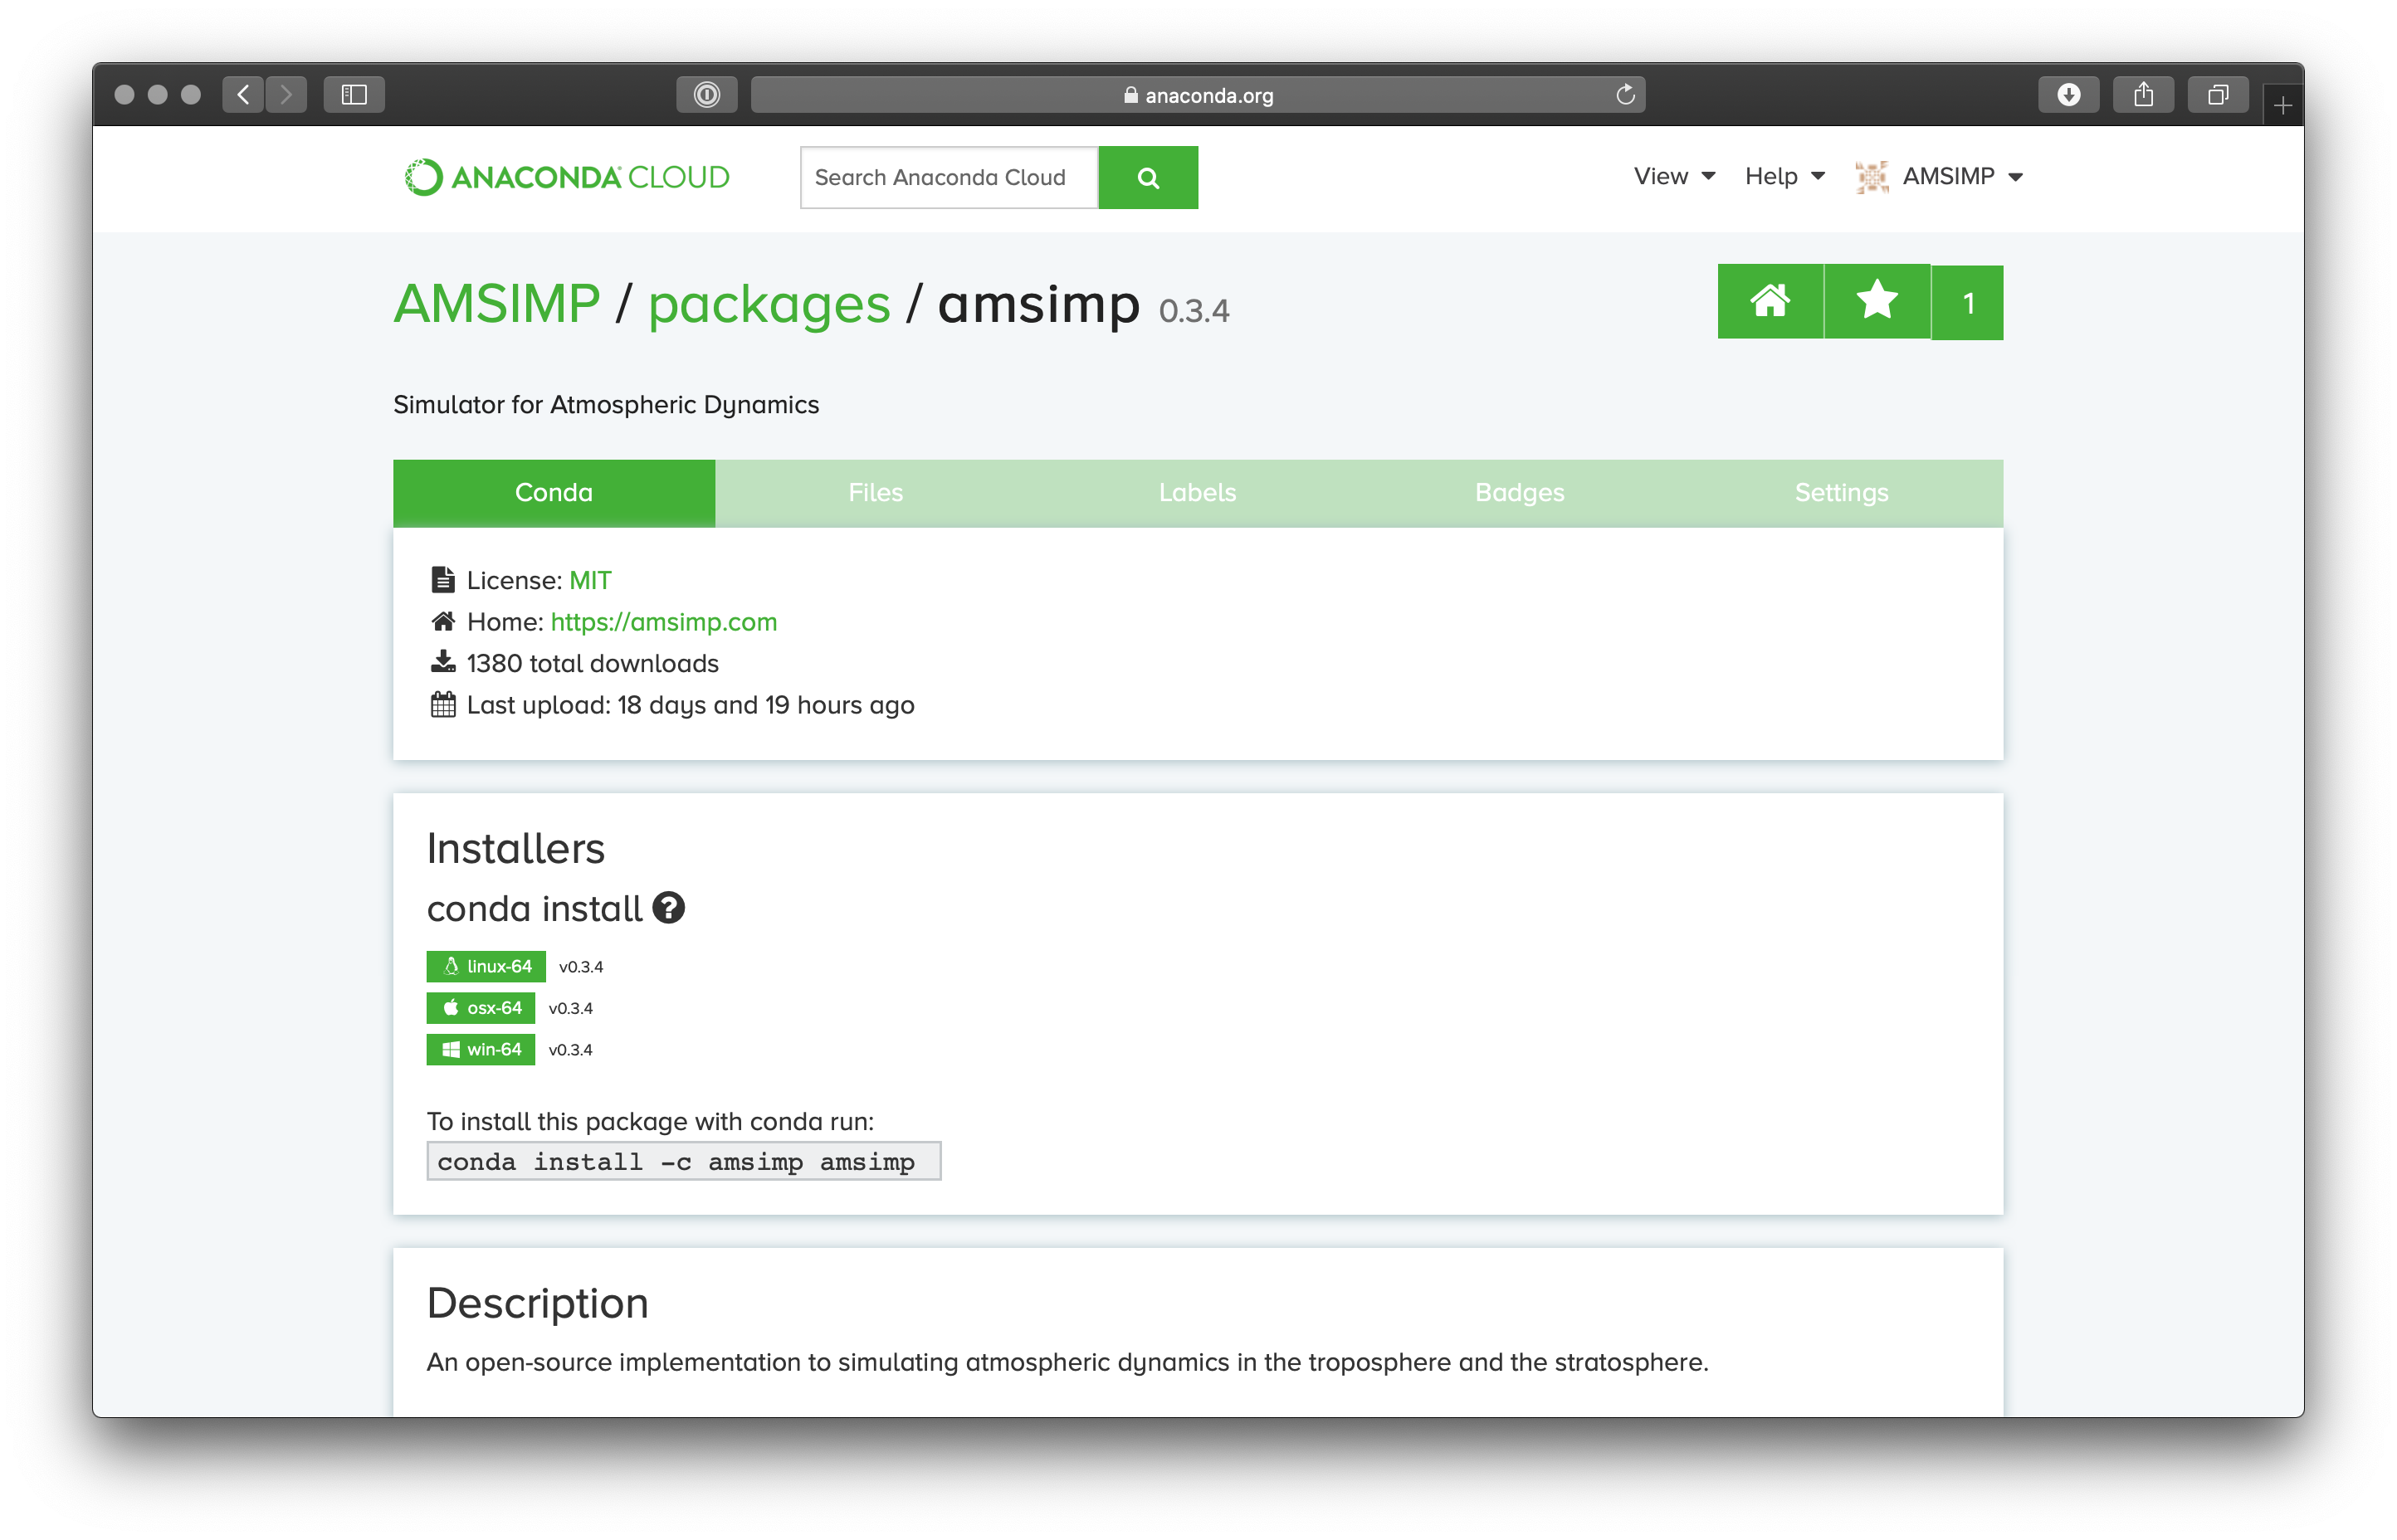
\includegraphics[width=.8\linewidth]{Images/anaconda.png}
    \caption{A screenshot of the AMSIMP package on Anaconda Cloud.}
    \label{pypi}
\end{figure}

While the hypothesis that was proposed has been proven, there is a few possible sources of error in the benchmarking method:

\begin{itemize}
    \item The accuracy benchmark was carried out over the course of a month (Mid November to Mid December). While the benchmark demonstrated that the forecast produced by the software was accurate, one might argue that due to the fact that it wasn't tested in the month of June, for example, that it is unknown whether the forecast produced by the software is accurate for the entirety of the year. Therefore, in the future, the accuracy benchmark would be carried out over a longer period of time in order to get a better picture in regards to the overall accuracy of the software.
    \item As mentioned in chapter \ref{5}, there is considerable debate as to whether there is a fixed cut off point for the mean and median absolute percentage errors. The reason one might argue is the fact that MAPE / MdAPE is levelled. Therefore, a potential remedy to this is, to switch to the mean absolute scaled error, which has a definite cut off point of 1. Problems with the MAPE and MdAPE can also occur when calculating them with a series of small denominators.  A singularity problem of the form `one divided by zero' and the creation of very large changes in the Absolute Percentage Error, caused by a small deviation in error, can occur.
    \item It is necessary to point out at this stage that the linting benchmark, which is a specific code quality benchmark, was carried out on AMSIMP v0.1.6, while all other benchmarks were carried out on the latest version of the software, AMSIMP v0.3.4. The reason for doing so is that Pylint is currently incompatible with Cython, and there is currently no similar linter available for this programming language. While the functionality of both versions is similar, with the source code being practically identical for all intents and purposes; it is still something to emphasise, and keep in mind.
\end{itemize}

\section{Looking Ahead}
The software is currently in a beta release state. Beta software is generally considered ``complete" by the developer but still not ready for general use due to a lack of testing ``in the wild."\cite{beta}. In this section, I will briefly outline the enhancements and features that will be released in the release candidate version of the software, which is planned for release in Fall 2020:

\begin{itemize}
    \item The next fundamental step for the project will be utilising live, or near to it, atmospheric data in order to provide a forecast that is of a higher accuracy, and as a consequence, would be more useful to the general population. For the purposes of this project, the data used was provided by the NRLMSISE-00 Atmospheric Model. During the research phase of the project, it was discovered that the data provided by this model had a mean absolute percentage error of approximately 1.5 \% and a median absolute percentage error of approximately 0.8 \%. While one might argue that this is reasonable accurate, as a consequence of Chaos Theory, a tiny difference in the initial conditions in a large system can result in drastically different forecasted events. One can determine a system's sensitivity to initial conditions by utilising the Lyapunov exponent. The Lyapunov exponent can be determined by equation \ref{chaos}, where in this $e$ is Euler's number and $\lambda$ is the Lyapunov exponent \cite{lyapunov}.
    
    \begin{equation}
        \label{chaos}
        \mid{\delta Z(t)}\mid \approx e^{\lambda t} \mid{\delta Z_{0}}\mid
    \end{equation}
    
    It cannot be determined analytically, similar to the Primitive Equations, and must be calculated numerically. If one determines its value, it would demonstrate that the atmosphere is a system that is extremely sensitive to initial conditions. Such a system is known as a chaotic dynamical system. Hence, while utilising live atmospheric data would add a significant amount of complexity, it would greatly improve the accuracy of the forecast produced by the software.
    \item A key assumption that is held to be true within the software, and by extension the project, is that the atmosphere is in geostrophic balance. While this is a reasonably good approximation at a synoptic scale, especially in the  mid-latitude mid-troposphere, it generally does not hold true in nature. The actual wind always differs from the geostrophic wind due to forces from surface level, such as friction. Thus, the actual wind would equal the geostrophic wind if there was no friction and the isobars were pretty straight. For release candidate version of the software, the current plan is to implement the Quasi-geostrophic theory into the software. The Quasi-geostrophic are used to model flows in the atmosphere more widely. These theories allow for divergence to take place and for weather systems to then develop\cite{quasi_future}.
    \item The aforementioned features will be released in the AMSIMP v1.0.0, which as stated previously is planned for release in the Fall of 2020. Dependent on demand and utilisation of the software, and in the hopes of making the software more generally available and accessible to a wide audience of people; an app, most likely for iOS, will be created and would coincide with the launch of AMSIMP v2.0.0, which at this present moment is slated for release in the Summer of 2021.
\end{itemize}